\documentclass[a4paper,14pt]{extarticle}%Формат бумаги А4, 14 кегль.


\usepackage{extsizes}
\usepackage{cmap} % для кодировки шрифтов в pdf
\usepackage[T2A]{fontenc}
\usepackage[utf8]{inputenc}
\usepackage[russian]{babel}%Языки используемые в документе
\usepackage{ucs}
\usepackage[pdftex]{graphicx} % для вставки картинок
\graphicspath{{images/}}%Папка с изображениями
\DeclareGraphicsExtensions{.pdf,.png,.jpg,.bmp}%Установка форматов изображений


\usepackage[nooneline]{caption}% Переопределение заголовков рисунков и таблиц
%\RequirePackage{caption}
	\DeclareCaptionLabelSeparator{defffis}{ -- }%Установка дефиса
	

\captionsetup[table]{labelsep=defffis,justification=raggedright,singlelinecheck=false,font=normalsize}
\captionsetup[figure]{justification=centering,labelsep=defffis,name=Рисунок} 






\usepackage{floatrow} % плавающие обьекты, крутые оформления названий рисунков и тп.
\floatsetup[table]{style=Plaintop} %Название таблицы сверху
\usepackage{setspace} 
\usepackage{pdfpages} %для вставки пдф страниц
\usepackage{longtable} % Подключение переносимых автоматически таблиц
\usepackage{amssymb,amsfonts,amsmath,amsthm} % математические дополнения от АМС
\usepackage{indentfirst} % отделять первую строку раздела абзацным отступом тоже
\usepackage[usenames,dvipsnames]{color} % названия цветов
\usepackage[table,xcdraw,hyperref]{xcolor} %цвета
\usepackage{makecell}
\usepackage{multirow} % улучшенное форматирование таблиц
\usepackage{ulem} % подчеркивания
\usepackage{import}% Импорт файлов
\usepackage{float} % Расширенное управление плавающими объектами




% список сокращений
\usepackage{nomencl} 
%\usepackage{etoolbox} %Нужна для настройки списков

%Настройка списков
%\renewcommand\nomgroup[1]{%
%  \item[\bfseries
%  \ifstrequal{#1}{T}{Определения}{%
%  \ifstrequal{#1}{O}{Обозначения и сокращения}{}}%
%]}






%Графики и схемы
\usepackage{tikz} % Рисование графиков и тд.
%\usetikzlibrary{graphs}
% Блок-схема определяет основную форму
\tikzstyle{main} = [rectangle, rounded corners, minimum width = 2cm, minimum height=1cm,text centered, draw = black]
 % Форма стрелки
\tikzstyle{arrow} = [ultra thick,->,>=stealth]

% Графики функций
\usepackage{pgfplots}
\pgfplotsset{compat=1.9}



% Определение размеров полей
\usepackage{geometry}
	\geometry{left=3cm}
	\geometry{right=1.5cm}
	\geometry{top=2cm}
	\geometry{bottom=2cm}
		
%Установка шрифтов
\usepackage{xltxtra} % fontspec %пакет хелатех для таймс нью роман
%\setmainfont{Arial} % таймс нью роман
\setmainfont{Times New Roman} % таймс нью роман
\defaultfontfeatures{Ligatures=TeX,Mapping=tex-text}

\frenchspacing
\pagestyle{plain}
\linespread{1.4} % полуторный интервал
\setlength{\parindent}{1.27cm} % Абзацный отступ
\setlength{\parskip}{0pt}
\sloppy % указывает, что с залезанием слов на поля следует бороться, даже применяя недопустимо длинные пробелы.

\usepackage{hyperref} %Ссылки
\definecolor{linkcolor}{HTML}{000000} % цвет ссылок (черный)
\definecolor{urlcolor}{HTML}{0000ff} % цвет гиперссылок


%Библиография
\usepackage[square,numbers,sort&compress]{natbib}
\renewcommand{\bibnumfmt}[1]{#1.\hfill} % нумерация источников в самом списке — через точку
\renewcommand{\bibsection}{\centering{\section*{Список использованных источников}}} % заголовок специального раздела
\setlength{\bibsep}{0pt}
%\bibliographystyle{gost780u}


\usepackage{tocloft} %регулировка расположения TableOfContent (Оглавления) на странице
% % Отточия в Оглавлении
%\renewcommand\cftchapdotsep{\cftdot} %добавляет отточия после \chapter{title}
\renewcommand\cftsecdotsep{\cftdot} %делает отточия после \section{title} частыми.



\makeatletter
\renewcommand{\l@section}{\@dottedtocline{1}{0em}{1.25em}}
\renewcommand{\l@subsection}{\@dottedtocline{2}{1.25em}{1.75em}}
\renewcommand{\l@subsubsection}{\@dottedtocline{3}{2.75em}{2.6em}}
\makeatother



%GGWP мне ебал мозг с требованием по отступу между заголовком и основным текстом, если вдруг кто-то начнет titlespacing надо раскоментить. Тогда надо поменять значения размера шривта в titleformat везде на \normalfont или \large(С ним опасно, но если ориентироваться на госты можно, единственное, что сраться прийдется)

\usepackage{titlesec}    

%%\titlespacing{\crapter}{0pt}{1.4pt}{1.4pt}
%\titlespacing{\section}{0pt}{1.4pt}{1.4pt}
%\titlespacing{\subsection}{0pt}{1.4pt}{1.4pt}
%\titlespacing{\subsubsection}{0pt}{1.4pt}{1.4pt}

%\titleformat{\crapter}[block]{\filcenter}{\centering}{\thesection}{\textbf}
\titleformat{\section}[block]{\Large\bfseries\filcenter}{\shape\thesection}{1em}{}
\titleformat{\subsection}[block]{\large\normalfont\bfseries\filcenter}{\shape\thesubsection}{1em}{}
\titleformat{\subsubsection}[block]{\normalfont\bfseries\filcenter}{\shape\thesubsubsection}{1em}{}
\titleformat{\paragraph}[block]{\normalfont\bfseries}{\shape\theparagraph}{1em}{}
\titleformat{\subparagraph}[runin]{\normalfont\bfseries}{\shape\thesubparagraph}{1em}{}


%\renewcommand{\aftersection}{6pt plus .1pt}

%Списки

%Настройка отступов в списках enumerate
\makeatletter
\let\old@enumerate=\enumerate
\def\enumerate{\old@enumerate
\setlength{\itemsep}{0pt}
\setlength{\parskip}{0pt}
\setlength{\leftskip}{0pt}
}\makeatother


%Настройка отступов в списках itemize
%\makeatletter
%\let\old@itemize=\itemize
%\def\itemize{\old@itemize
%\setlength{\itemsep}{0pt}
%\setlength{\parskip}{0pt}
%\setlength{\leftskip}{0pt}
%\makeatother

%маркеры списков
%\renewcommand{\labelitemi}{--}      % Маркер списка --
%\renewcommand{\labelenumi}{--}      % Список второго уровня
%\renewcommand{\labelenumii}{--}     % Список третьего уровня
    %\renewcommand{\labelenumi}{\asbuk{enumi})}    % Список второго уровня
    %\renewcommand{\labelenumii}{\arabic{enumii})} % Список третьего уровня
%Нумерация цифрами
\renewcommand{\labelenumii}{\arabic{enumi}.\arabic{enumii}.}



\usepackage{circuitikz} %преамбула
% Оглавление
\newcommand{\mtableofcontents}{
\thispagestyle{empty}
    \begin{center}
		\tableofcontents
	\end{center}
\newpage}

%ОПРЕДЕЛЕНИЯ, ОБОЗНАЧЕНИЯ И СОКРАЩЕНИЯ
%Перечень сокращений и обозначений
%Не работает корректно
% Список сокращений
%Определения, обозначения и сокращения
\newcommand{\sokraseniya}{
    \thispagestyle{empty}
    \renewcommand{\nomname}{Перечень сокращений и обозначений}
    \makenomenclature
    \addcontentsline{toc}{section}{Перечень сокращений и обозначений}
    \newcommand*{\nom}[2]{##1\nomenclature{##1}{##2}}
    \begin{center} \printnomenclature[5em] \newpage \end{center}
}


%\newcommand{\sokraseniya}{
%    \thispagestyle{empty}
%    \section*{Перечень сокращений и обозначений}
%    \addcontentsline{toc}{section}{Перечень сокращений и обозначений}
%    % Пример оформления
%\nomenclature{ЭС}{Электронные средства}
%\nomenclature{}{}
%Термины, определения и сокращения




    %
    %Определения
    %

    %\nomenclature[T]{Джиттер}{jitter, Дрожание фазы, Отклонение фазы или частоты сигнала}

    %
    % Обозначения и сокращения
    %

    \nomenclature{ППМ}{Приемо-передающий модуль}
    \nomenclature{АФАР}{Активная фазированная антенная решетка}
    \nomenclature{ОКР}{Опытно-конструкторская разрабоотка}
    

%\hypertarget{dc}{ЦОД --- центр обработки данных}


%    \newpage
%}


\newcommand{\data}{«\begin{tikzpicture}\draw(0,0) -- (0.7,0);\end{tikzpicture}»\begin{tikzpicture}\draw(0,0) -- (1.5,0);\end{tikzpicture} \the\year{} г.}


%
%\renewcommand{\appendix}{\renewcommand{\thesection}{Приложение \Asbuk{section}}\newcommand{\appsec}{\newpage\section{}\setcounter{page}{1}}} % сокращения больших конструкций
\newcommand{\analogone}{ZK-CLOCK (TL082)}
\newcommand{\analogtwo}{M16} 
\newcommand{\analogthree}{UDB1008S}
\newcommand{\analogfour}{HBKS} 
\newcommand{\analogfive}{MHS-5200P}
\newcommand{\analogsix}{UDB1108S}

\newcommand{\assemblyblueprint}{МРАГ.467872.001СБ}
\newcommand{\shemblueprint}{МРАГ.467872.001ЭЗ}
\newcommand{\psbblueprint}{МРАГ.758752.001ПП}
\newcommand{\spekblueprint}{МРАГ.467872.001} % переменные (для удобства работы с текстом)


\setcounter{page}{1}% С какой страницы начать отсчёт

%\includepdf[pages = {1, 3-7}]{sections/tituls.pdf} для вставки ПДФ страниц (титульников например)
%\footnote{АФЧХ - амплитудно-фазовая частотная характеристика, диаграмма или годограф Найквиста(Nyquist Plot), частотный отклик системы(frequency response).} Сноска



\begin{document}
\thispagestyle{empty}

\begin{center}
\begin{spacing}{1}

\begin{figure}[H]
    \centering
    
\includegraphics{images/titul/1.png} %[width=0.15\linewidth]
\end{figure}


        \small МИНОБРНАУКИ РОССИИ\\
        \small Федеральное государственное бюджетное образовательное учреждени\\
        \small высшего образования\\
        \small \textbf{«МИРЭА – Российский технологический университет}»\\
        \Large\textbf{РТУ МИРЭА}
        \vspace{0cm}
        
    \begin{tikzpicture}
    \draw(0,0) -- (15,0);
    \draw(0,0.1) -- (15,0.1);
    \end{tikzpicture}



        \normalsize  Филиал РТУ МИРЭА в г. Фрязино\\
        \normalsize Базовая кафедра №143 – конструирования СВЧ и цифровых радиоэлектронных средств\\
        
        \vspace{0.5cm} 
        
        \Large\textbf{КУРСОВАЯ РАБОТА}\\
        \normalsize по дисциплине\\
        \normalsize <<Основы теории радиоэлектронных устройств>>\\
        \textbf{Тема курсовой работы: «ППМ для АФАР Х-диапазона с предельно низким уровнем боковых лепестков: -50 dB»}

        \vspace{2cm}


    \begin{flushleft} Студент группы: \hspace{0.5cm} \underline{ФКМО-01-22} \hspace{2cm} Бадулин Д.Р. \end{flushleft}
    \vspace{0.3cm}
    \begin{flushleft} Руководитель курсового проекта \hspace{2cm} Куприянов П.В. \end{flushleft}
    \begin{flushleft} Профессор, д.т.н.	 \end{flushleft}
    \vspace{0.3cm}
    \begin{flushleft} Рецензент \end{flushleft}
    \vspace{0.5cm}
    \begin{flushleft} Работа представлена к защите \hspace{0.3cm}  \data \end{flushleft}
    \vspace{0.5cm}
    \begin{flushleft} Допущен к защит \hspace{0.3cm}   \data \end{flushleft}
    \vspace{2cm}


\normalsize Фрязино \the\year{}
\end{spacing}
\end{center}


\newpage
\thispagestyle{empty} 

\begin{center}
\begin{spacing}{1}
    \begin{figure}[H]
        \centering
        
\includegraphics{images/titul/1.png} %[width=0.15\linewidth]
    \end{figure}


    \small МИНОБРНАУКИ РОССИИ\\
    \normalsize Федеральное государственное бюджетноеобразовательное учреждени\\
    \normalsize высшего образования\\
    \normalsize \textbf{«МИРЭА – Российский технологический университет}»\\
    \Large\textbf{РТУ МИРЭА}\\
        
    \begin{tikzpicture}
    \draw(0,0) -- (15,0);
    \draw(0,0.1) -- (15,0.1);
    \end{tikzpicture}




    \normalsize  Филиал РТУ МИРЭА в г. Фрязино\\
    \normalsize Базовая кафедра №143 – конструирования СВЧ и цифровых радиоэлектронных средств\\
    
    

    \begin{flushright}
        \small    \textbf{Утверждаю}\\
        \footnotesize    Заведующий кафедрой\\
        \footnotesize    Щербаков С.В.\\
        \footnotesize    \data
    \end{flushright}

    
    
    \large \textbf{ЗАДАНИЕ}\\
    \normalsize \textbf{на выполнение курсовой работы}\\
    \normalsize \textbf{по дисциплине «Основы теории радиоэлектронных устройств»}
    
    
    
    \end{spacing}
\end{center}

\begin{spacing}{1}
    \begin{enumerate}
        %\normalsize
        \footnotesize \item \textbf{Тема «ППМ для АФАР Х-диапазона с предельно низким уровнем боковых лепестков: -50 dB»}
        
        \item \textbf{Исходные данные:}\\
        Уровень боковых лепестков: -50 дБ.
        
        \item  \textbf{Перечень вопросов, подлежащих разработке, и обязательного графического материала:}
         %\footnotesize
        Техническое задание на научно-исследовательскую работу, ТЗ должно включать в себя: 
        
требования назначения, требования живучести, требования надежности и стойкости к внешним воздействиям, требования гамма-процентной наработки до отказа, требования наработки до отказа всей системы 1000 часов (2000 модулей в системе), требования технологичности: применяемые технологии, описание как подается питание физически, протокол управления; требования к документации.
        
        \item \textbf{Срок представления к защите курсового проекта:\\ до}  \data
    \end{enumerate}
    

    \begin{table}[H]
        \flushleft
        \begin{tabular}{ll}
            \begin{tabular}{l}
            \footnotesize    Задание на курсовую\\ \footnotesize работу выдал
            \end{tabular} & \footnotesize \data\\
            
            \begin{tabular}{l}
            \footnotesize    Задание на курсовую\\ \footnotesize работу получил
            \end{tabular} & \footnotesize \data\\
        
        \end{tabular}
    \end{table}
  
  
  
  \begin{center}
    \normalsize   Фрязино \the\year{}
  \end{center}
  
\end{spacing}
\newpage
%\input{sections/titul}
\pagestyle{empty}
    \begin{center}
        \tableofcontents
    \end{center}
	\newpage
    \pagestyle{plain}
\sokraseniya % Команда на генерацию списка сокращений
% Пример оформления
%\nomenclature{ЭС}{Электронные средства}
%\nomenclature{}{}
%Термины, определения и сокращения




    %
    %Определения
    %

    %\nomenclature[T]{Джиттер}{jitter, Дрожание фазы, Отклонение фазы или частоты сигнала}

    %
    % Обозначения и сокращения
    %

    \nomenclature{ППМ}{Приемо-передающий модуль}
    \nomenclature{АФАР}{Активная фазированная антенная решетка}
    \nomenclature{ОКР}{Опытно-конструкторская разрабоотка}
    

%\hypertarget{dc}{ЦОД --- центр обработки данных}

 % список терминов и сокращений
\begin{center}
\section*{Введение}
\end{center}
\addcontentsline{toc}{section}{Введение}



%Актуальность

%Про эту штуку

%Фишки






%Цели



%Задание




%Задачи


 %введение
\newpage
\section{Основная информация о ОКР}


\paragraph{Наименование} ППМ для АФАР Х-диапазона с предельно низким уровнем боковых лепестков: -50 dB.


\paragraph{Шифр ОКР}


ШИФР




\paragraph{Основание постановки работы}

Основанием постановки работы является задание на курсовую работу в рамках предмета основы теории радио-электроных устройств. Задание на курсовую работу выдано профессором филиала РТУ МИРЭА в городе Фрязино Куприяновым П.В.




\paragraph{Исполнитель}

Студент группы: ФКМО-01-22 Бадулин Д.Р.



\paragraph{Сроки выполнения}

Вчера

\paragraph{Цель ОКР, наименование и обозначение изделия}

Разработать ППМ для АФАР Х-диапазона с предельно низким уровнем боковых лепестков: -50dB.

 %Аналитический обзор
\section{Технические требования}

\subsection{Требования назначения}

Требования к электрическим параметрам изделия представлены в таблице \ref{tab:teh-treb-ez}.




\begin{longtable}{|p{4cm}|p{2cm}|p{2cm}|p{2cm}|p{2cm}|p{2cm}|}
\caption{Требования к электрическим параметрам изделия}\label{tab:teh-treb-ez}
\hline
\multirow{2}{4cm}{\textbf{Параметр}}                   & \multirow{2}{2cm}{\textbf{Обознач-ение}}    & \multicolumn{3}{c|}{\textbf{Норма}} & \multirow{2}{2cm}{\multicolumn{1}{c}{\textbf{Примечание}}} \\ \cline{3-5}
& & \textbf{Не менее} & \textbf{Номинал} & \textbf{Не более} & \\ \hline 
\endfirsthead    % Первые ячейки начала таблицы
\caption*{Продолжение таблицы \ref{tab:teh-treb-ez}}%
\hline
\multirow{2}{4cm}{\textbf{Параметр}}                   & \multirow{2}{2cm}{\textbf{Обознач-ение}}    & \multicolumn{3}{c|}{\textbf{Норма}} & \multirow{2}{2cm}{\multicolumn{1}{c}{\textbf{Примечание}}} \\ \cline{3-5}
& & \textbf{Не менее} & \textbf{Номинал} & \textbf{Не более} & \\ \hline 
\endhead %первые ячейки после каждого переноса на новую строку
Диапазон рабочих частот, ГГц & $\Delta f_\text{раб.}$ &  & & & \\ 
-- Нижняя граница & & 8 & & & \\ 
-- Номинал & & & Не нормируется & & \\ 
-- Верхняя граница & & & & 12 & \\ \hline 
Диапазон частот выходного сигнала, полоса частот, МГц & $\Delta f_\text{вых.}$ & 300 & 500 & 700 & \\ \hline
Диапазон регулировки фазы, ° &  & 0 & Не нормируется & 360 & \\
Шаг регулировки фазы, ° &  & 10 & 11 & 12 & \\
Точностью установки фазы, ° &  & 5 & 8 & 20 & \\ \hline
Коэффициент передачи, дБ & $K_\text{пер.}$ & 30 & 32 & 35 & \\ \hline
Коэффициент шума, дБ & $K_\text{ш}$ & Не нормируется & 4 & 10 & \\ \hline
Неравномерность коэффициента передачи, дБ & $\Delta K_\text{пер.}$ & - & - & 3 & \\ \hline
%Мгновенный динамический диапазон в режиме <<узкая полоса>>(при компрессии $K_\text{пер.} = 1$ дБ), дБм & $\text{ДД}_\text{мги}$ & 85 & - & - & (75 - максимальное значение)\\ \hline
Верхняя граница линейности амплитудной характеристики по выходу полосы частот (при компрессии $K_\text{пер.} = 1$ дБ), дБм & $P_\text{лин. вых.}$ & 26 & 28 & 30 &  \\ \hline

\end{longtable}


Протокол управления: SPI; Количество каналов управления: 4; Уровни управляющих сигналов: 1,8 и(или) 3,3; 




\subsection{Требования живучести}

Обеспечить сохранение работоспособности изделия в течении всего срока службы, срок службы изделия определяется документацией.

\subsection{Требования надежности}

Наработка до отказа системы из двух тысяч модулей - 1000 часов.


\subsection{Требования стойкости к климатическим воздействиям}

Настоящее изделие согласно \textit{ГОСТ-15150-69} относится к категории \textit{W5.1}. Категория \textit{W5.1} - это изделия, предназначенные для эксплуатации во всех макроклиматических районах на суше и на море, кроме климатического района с антарктическим холодным климатом (всеклиматическое исполнение). Для эксплуатации в качестве встроенных элементов внутри комплектных изделий, предназначенных для эксплуатации в помещениях (объемах) с повышенной влажностью (например, в неотапливаемых и невентилируемых подземных помещениях, в том числе шахтах, подвалах, в почве, в таких судовых, корабельных и других помещениях, в которых возможно длительное наличие воды или частая конденсация влаги на стенах и потолке, в частности в некоторых трюмах, в некоторых цехах текстильных, гидрометаллургических производств и т.п.), конструкция которых исключает возможность конденсации влаги на встроенных элементах (например, внутри радиоэлектронной аппаратуры).\cite{GOST-1}


Требуемые значения рабочих температур представлены в таблицах \ref{tab:treb-temp-shadow}, \ref{tab:treb-temp-solar}.

\begin{table}[H]
    \centering
    \begin{tabular}{|c|c|c|c|}
    \hline
    \multicolumn{2}{|c|}{\textbf{Рабочая температура}} & \multicolumn{2}{c|}{\textbf{Предельная рабочая температура}}\\ \hline
       \textbf{Верхний предел} & \textbf{Нижний предел} & \textbf{Верхний предел} & \textbf{Нижний предел} \\ \hline
       \multicolumn{1}{|c|}{$+45^\circ C$}& $-40^\circ C$ & $+45^\circ C$ & $-40^\circ C$ \\ \hline
    \end{tabular}
    \caption{Требуемые рабочие температуры в тени}
    \label{tab:treb-temp-shadow}
\end{table}




\begin{table}[H]
    \centering
    \begin{tabular}{|c|c|c|c|}
    \hline
    \multicolumn{2}{|c|}{\textbf{Рабочая температура}} & \multicolumn{2}{c|}{\textbf{Предельная рабочая температура}}\\ \hline
       \textbf{Верхний предел} & \textbf{Нижний предел} & \textbf{Верхний предел} & \textbf{Нижний предел} \\ \hline
    $+60^\circ C$ & $-25^\circ C$ & $+60^\circ C$ & $-25^\circ C$ \\ \hline
    \end{tabular}
    \caption{Требуемые рабочие температуры под воздействием солнечного излучения}
    \label{tab:treb-temp-solar}
\end{table}


Требования к рабочей влажности воздуха представлены на таблице \ref{tab:rab-vlaj-vozd}.

\begin{table}[H]
    \centering
    \begin{tabular}{|l|l|p{7cm}|}
        \hline
         \textbf{Средне годовая} & \textbf{Верхнее значение} & \textbf{Абсолютная влажность среднегодовое значение} \\ \hline
         \multicolumn{1}{|c|}{ 80\% при $27^\circ C$ } & \multicolumn{1}{c|}{98\% при $35^\circ C$} & \multicolumn{1}{c|}{20}\\ \hline 
    \end{tabular}
    \caption{Требования к рабочей влажности воздуха}
    \label{tab:rab-vlaj-vozd}
\end{table}

Требования к атмосферному давлению представлены в таблице \ref{tab:treb-davl}.

\begin{table}[H]
    \centering
    \begin{tabular}{|c|c|}
    \hline
        \multicolumn{2}{|c|}{\textbf{Атмосферное давление, \[кПа\]}}  \\ \hline
        \textbf{Верхний предел} & \textbf{Нижний предел} \\ \hline
        106,7 & 84,0 \\ \hline
    \end{tabular}
    \caption{Требования к давлению воздуха в процессе работы устройства}
    \label{tab:treb-davl}
\end{table}

\subsection{Требования к технологичности}

Технологические ограничения к параметрам печатной платы представлены в таблице \ref{tab:teh-treb-pp}. Допустимые материалы печатной платы:




\begin{itemize}
    \begin{minipage}{.30\textwidth}
        \item FR-4;
        \item RO4003C;
        \item RO4350B;
        \item WL-CT338;
    \end{minipage}
    \begin{minipage}{.30\textwidth}
        \item WL-CT350;
        \item F4BM255;
        \item WL-PP350.
    \end{minipage}
\end{itemize}





\begin{longtable}{|p{5cm}|p{2cm}|p{3cm}|p{4cm}|}
\caption[123]{Ограничения к параметрам печатной платы}\label{tab:teh-treb-pp}
\hline
\textbf{Параметр}                    & \textbf{Толщина металлизации} & \textbf{Нижний предел, мм} & \textbf{Верхний предел, мм}  \\ \hline
\endfirsthead    % Первые ячейки начала таблицы
\caption*{Продолжение таблицы \ref{tab:teh-treb-pp}}%
\hline
\textbf{Параметр}                    & \textbf{Толщина металлизации} & \textbf{Нижний предел, мм} & \textbf{Верхний предел, мм}  \\ \hline
\endhead %первые ячейки после каждого переноса на новую строку
\multirow{4}{5cm}{Ширина проводника} & 18                            & 0,125                      & Не нормируется \\ \cline{2-4}
                                   & 35                            & 0,200                        & Не нормируется \\ \cline{2-4}
                                   & 70                            & 0,300                        & Не нормируется \\ \cline{2-4}
                                   & 105                           & 0,350                       & Не нормируется \\ \hline
\multirow{4}{5cm}{Зазор между проводниками} & 18                     & 0,125                      & Не нормируется \\ \cline{2-4}
                                   & 35                            & 0,200                        & Не нормируется \\ \cline{2-4}
                                   & 70                            & 0,300                        & Не нормируется \\ \cline{2-4}
                                   & 105                           & 0,350                       & Не нормируется \\ \hline
\multirow{4}{5cm}{Ширина проводника спирального типа}
& 18                            & 0,200                      & Не нормируется \\ \cline{2-4}
                                   & 35                            & 0,250                        & Не нормируется \\ \cline{2-4}
                                   & 70                            & 0,300                        & Не нормируется \\ \cline{2-4}
                                   & 105                           & 0,350                       & Не нормируется \\ \hline
\multirow{4}{5cm}{Зазор между проводниками спирального типа} & 18                     & 0,120                      & Не нормируется \\ \cline{2-4}
                                   & 35                            & 0,250                        & Не нормируется \\ \cline{2-4}
                                   & 70                            & 0,300                        & Не нормируется \\ \cline{2-4}
                                   & 105                           & 0,350                       & Не нормируется \\ \hline
\multirow{4}{5cm}{Зазор между полигоном и элементами остальной топологии}& 18                     & 0,200                      & Не нормируется \\ \cline{2-4}
                                   & 35                            & 0,200                        & Не нормируется \\ \cline{2-4}
                                   & 70                            & 0,300                        & Не нормируется \\ \cline{2-4}
                                   & 105                           & 0,350                       & Не нормируется \\ \hline
\multirow{4}{5cm}{Параметры сетчатого полигона} & 18                     & 0,200                      & Не нормируется \\ \cline{2-4} 
                                   & 35                            & 0,200                        & Не нормируется \\ \cline{2-4}
                                   & 70                            & 0,300                        & Не нормируется \\ \cline{2-4}
                                   & 105                           & 0,350                       & Не нормируется \\ \hline
\multirow{4}{5cm}{Зазор между открытыми от маски элементами топологии при финишном покрытии ПОС-63} & 18                     & 0,200                      & Не нормируется \\
& & & \\ \cline{2-4}
                                   & 35                            & 0,250                        & Не нормируется \\ \cline{2-4}
                                   & 70                            & 0,300                        & Не нормируется \\ \cline{2-4}
                                   & 105                           & 0,350                       & Не нормируется \\ \hline
Металлизированное отверстие & --                     & 0,300                      & Не нормируется \\ \hline
Отступ элементов топологии от металлизированного отверстия на внутренних слоях & --                     & 0,250                      & Не нормируется \\ \hline
 Поясок монтажной контактной площадки & --                     & 0,200                      & Не нормируется \\ \hline
 Поясок площадки переходного отверстия & --                     & 0,150                      & Не нормируется \\ \hline
Отношение диаметра минимального металлизированного отверстия к толщине печатной платы & --                     & до 1:7, толщина ПП ≤ 2,5 мм                      & до 1:5, толщина ПП > 2,5 мм \\ \hline
Отношение глубины сверления к диаметру металлизированного отверстия & --                     & Не нормируется                      & Не нормируется \\ \hline
Диаметр межслойного переходного отверстия & -- & 0,300  & Не нормируется  \\ \hline

Минимальный диаметр монтажного отверстия & -- & 0,600  & Не нормируется \\ \hline
Диаметр металлизированного полуотверстия & -- & 0,600  & Не нормируется \\ \hline
Минимальное расстояние между краями двух отверстий & -- & 0,200  & Не нормируется \\ \hline
Неметаллизированное отверстие & -- & 0,500  & Не нормируется \\ \hline
Отступ элементов топологии от неметаллизированного отверстия на всех слоях & -- & 0,200  & Не нормируется \\ \hline
Отступ элементов топологии от фрезеруемых контуров на внешних слоях & -- & 0,250  & Не нормируется \\ \hline
Отступ элементов топологии от фрезеруемых контуров на внутренних слоях & -- & 0,250  & Не нормируется \\ \hline
Отступ элементов топологии от края печатной платы на внешних слоях при скрайбировании & -- & 0,400  & Не нормируется \\ \hline
Отступ элементов топологии от края печатной платы на внутренних слоях при скрайбировании & -- & 0,400  & Не нормируется \\ \hline
Минимальная толщина платы & -- & 0,200  & Не нормируется \\ \hline
Минимальная ширина линии маркировки & -- & 0,150  & Не нормируется \\ \hline
Минимальная высота шрифта маркировки & -- & 1  & Не нормируется \\ \hline
Вскрытие текста в маске по текстолиту шириной не менее & -- & 0,150  & Не нормируется \\ \hline
Вскрытие текста в маске по сплошному металлу шириной не менее & -- & 0,250  & Не нормируется \\ \hline
\end{longtable}

\subsection{Требования к документации}


\begin{enumerate}
    \item Вся документация должна соответствовать действующим стандартам ЕСКД, ЕСТД, ЕСПД;
\end{enumerate}


\subsection{Требования приемки работы}

Работа считается выполненной с момента выполнения последнего пункта данного перечня:

\begin{enumerate}
\item В течении 30 рабочих дней с момента подписания контракта исполнитель обязан согласовать заказчиком комплектность конструкторской, технологической, программной документации;
\subparagraph{Примечание:}
В комплект документации обязательно должны войти следующие документы:
    \begin{enumerate}
        \item Схема Е1;
        \item Схема Э3;
        \item Перечень компонентов к схеме Э3.\footnote{перечень компонентов выполняется в виде отдельного документа}
        \item Чертеж печатной платы;\footnote{выполняется согласно ГОСТ 2.417-91}
        \item Сборочный чертеж устройства;
        \item Спецификация;
    \end{enumerate}
\item В течении 60 рабочих дней с момента выполнения пункта 1 исполнитель обязан согласовать перечень отчетной документации с заказчиком;
\item В течении 10 рабочих дней с момента выполнения пункта 2 исполнитель обязан предоставить отчет о проделанной работе в свободной форме с приложенной отчетной документацией;
\item В течении 30 рабочих дней с момента выполнения пункта 3 исполнитель согласует перечень отчетной технологической документации;
\item В течении 10 рабочих дней с момента выполнения пункта 4 исполнитель предоставляет отчет заказчику о проделанной работе с приложенной технологической документацией;
\item В течении 60 рабочих дней с момента выполнения пункта 5 исполнитель производит пять опытных образцов;
\item В течении 10 рабочих дней с момента выполнения пункта 6 исполнитель оформляет и согласует методику проведения испытаний с заказчиком и требования к протоколу проведения испытаний;
\item В течении 20 рабочих дней с момента выполнения пункта 7 исполнитель проводит испытания опытных образцов;
\item В течении 10 рабочих дней с момента выполнения пункта 8 исполнитель предоставляет отчет о проделанной работе в свободной форме, к отчету прилагаются пять протоколов проведения испытаний и пять опытных образцов;
\item В течении 20 рабочих дней с момента выполнения пункта 9 исполнитель формирует комплект документации на изделие и предоставляет его заказчику.
\end{enumerate}

\paragraph{Примечание} 
В случае не выполнения пунктов из перечня в поставленный срок на исполнителя будут накладываться санкции, в соответствии с нормативными документами, .установленными заказчиком на момент подписания контракта.


\newpage
\begin{center}
		\subsection*{Заключение}
	\addcontentsline{toc}{section}{Заключение}
\end{center}


 %заключение
\newpage

\begin{thebibliography}{3}
\addcontentsline{toc}{section}{Список использованных источников}

%





\bibitem{GOST-1}
ГОСТ-15150-69. Машины, приборы и другие технические изделия
\bibitem{GOST-2}
ГОСТ-РВ15.203-2000. Система разработки и постановки продукции на производство. ПРОДУКЦИЯ ПРОИЗВОДСТВЕННО-ТЕХНИЧЕСКОГО НАЗНАЧЕНИЯ. Порядок разработки и постановки продукции на производство
\bibitem{GOST-3}
ГОСТ 23221-78. Модули СВЧ, блоки СВЧ. Термины, определения и буквенные обозначения.
\bibitem{GOST-4}
ГОСТ Р 55787—2013. УСТРОЙСТВА ДЛЯ РАДИОСВЯЗИ, РАДИОВЕЩАНИЯ И ТЕЛЕВИДЕНИЯ АНТЕННО-ФИДЕРНЫЕ.
%\bibitem{GOST-?}
%ГОСТ Р 55744-2013. Платы печатные. Методы испытаний физических параметров.
\bibitem{GOST-5}
ГОСТ 24375-80. РАДИОСВЯЗЬ. Термины и определения.
\bibitem{GOST-6}
ГОСТ 2.417-91. ПЛАТЫ ПЕЧАТНЫЕ. Правила выполнения чертежей.
\bibitem{statiya-1}

Акики Д. и др. Университет "Нотр-Дам", г. Триполи, Ливан. Снижение уровня боковых лепестков зеркальных антенн методом позиционирования металлических полосок в раскрыве. * \text{[}Электронный ресурс\text{]} url: \url{https://hi.booksc.eu/book/36545448/daff7f} (дата обращения \today) %* \text{[}Электронный ресурс\text{]} url: \url{https://pnd-st.ru/ot-chego-zavisit-uroven-bokovyh-lepestkov-sposoby-umensheniya/} (дата обращения \today)






\end{thebibliography}




 % список источников
\newpage
\appendix
\renewcommand{\thesection}{Приложение \Asbuk{section}}
\newcommand{\appsec}{\newpage\section{}\setcounter{page}{1}\setcounter{equation}{0}}
% Сбросил номер страницы, номер формулы

\appsec
\section*{Расчет гамма-процентной наработки на отказ}

Наработка на отказ рассчитывается по формуле \ref{app:equationone}.

\begin{equation}\label{app:equationone}
    T_0 = \frac{1}{\Lambda_\text{РЭУ}};
\end{equation}
Где $T_0$ - наработка на отказ, $\Lambda_\text{РЭУ}$ - суммарная интенсивность отказов РЭУ с учетом электрического режима и условий эксплуатации.  

Гамма-процентная наработка до отказа рассчитывается по формуле \ref{app:equationtwo}.

\begin{equation}
\label{app:equationtwo}
T_\Gamma = - \frac{ln\left(\frac{\gamma}{100}\right)}{\Lambda_\text{РЭУ}} = -T_{0}\times ln\left(\frac{\gamma}{100}\right);
\end{equation}Где $\gamma = 90$ - вероятность безотказной работы.

Исходя из условий: наработка на отказ комплекса из 2000 модулей: 1000 часов. Наработка на отказ одного модуля будет  $T_1 \approx 0,5$.


Гамма-процентная наработка до отказа одного модуля:

\begin{equation*}
	T_{\Gamma1} = -0,5 \times ln\left(\frac{90}{100}\right) = -0,52 ;
\end{equation*}

\appsec


\begin{figure}[H]
    \centering
    \fbox{
\begin{circuitikz} 
\draw (0,0) node[mixer, box only, anchor=east, fill=cyan](m){}
(m.west) node[inputarrow]{} to[short, -o] ++(m.west) node[right=-30]{$I_{(t)}$} ++(-0.8,0);
\draw (m.south) node[inputarrow,rotate=90]{} --
++(0,-0.7) node[oscillator, box, anchor=north, fill=cyan]{} -- ++ (0,-1.6) node[inputarrow,rotate=270]{} node[circulator, box, anchor=north, fill=cyan](fase){};
\draw (fase.e) node[right] {$90^\circ$};
\draw (0,-5) node[mixer, box only, anchor=east, fill=cyan](mm){}
(mm.west) node[inputarrow]{} to[short, -o] (-2,-5)
(mm.west) node[right=-60]{$Q_{(t)}$};
\draw (fase.s) -- (mm.n) node[inputarrow,rotate=270]{};
\draw (3,-2.5) node[adder, box only, anchor=east, fill=cyan](sum){}
(m.e);
\draw (m.e)  -|  (sum.n) node[inputarrow,rotate=270]{};
\draw (mm.e)  -|  (sum.s) node[inputarrow,rotate=90]{};
\draw (sum.e)  -- (4,-2.5)
 (4,-2.5) node[inputarrow]{};
\end{circuitikz}
    }
    \caption{Квадратурный модулятор}
%    \label{fig:my_label}
\end{figure}



%\newpage
%\pagestyle{empty}
%\setcounter{page}{1}% С какой страницы начать отсчёт
%\section*{Приложение Б}

%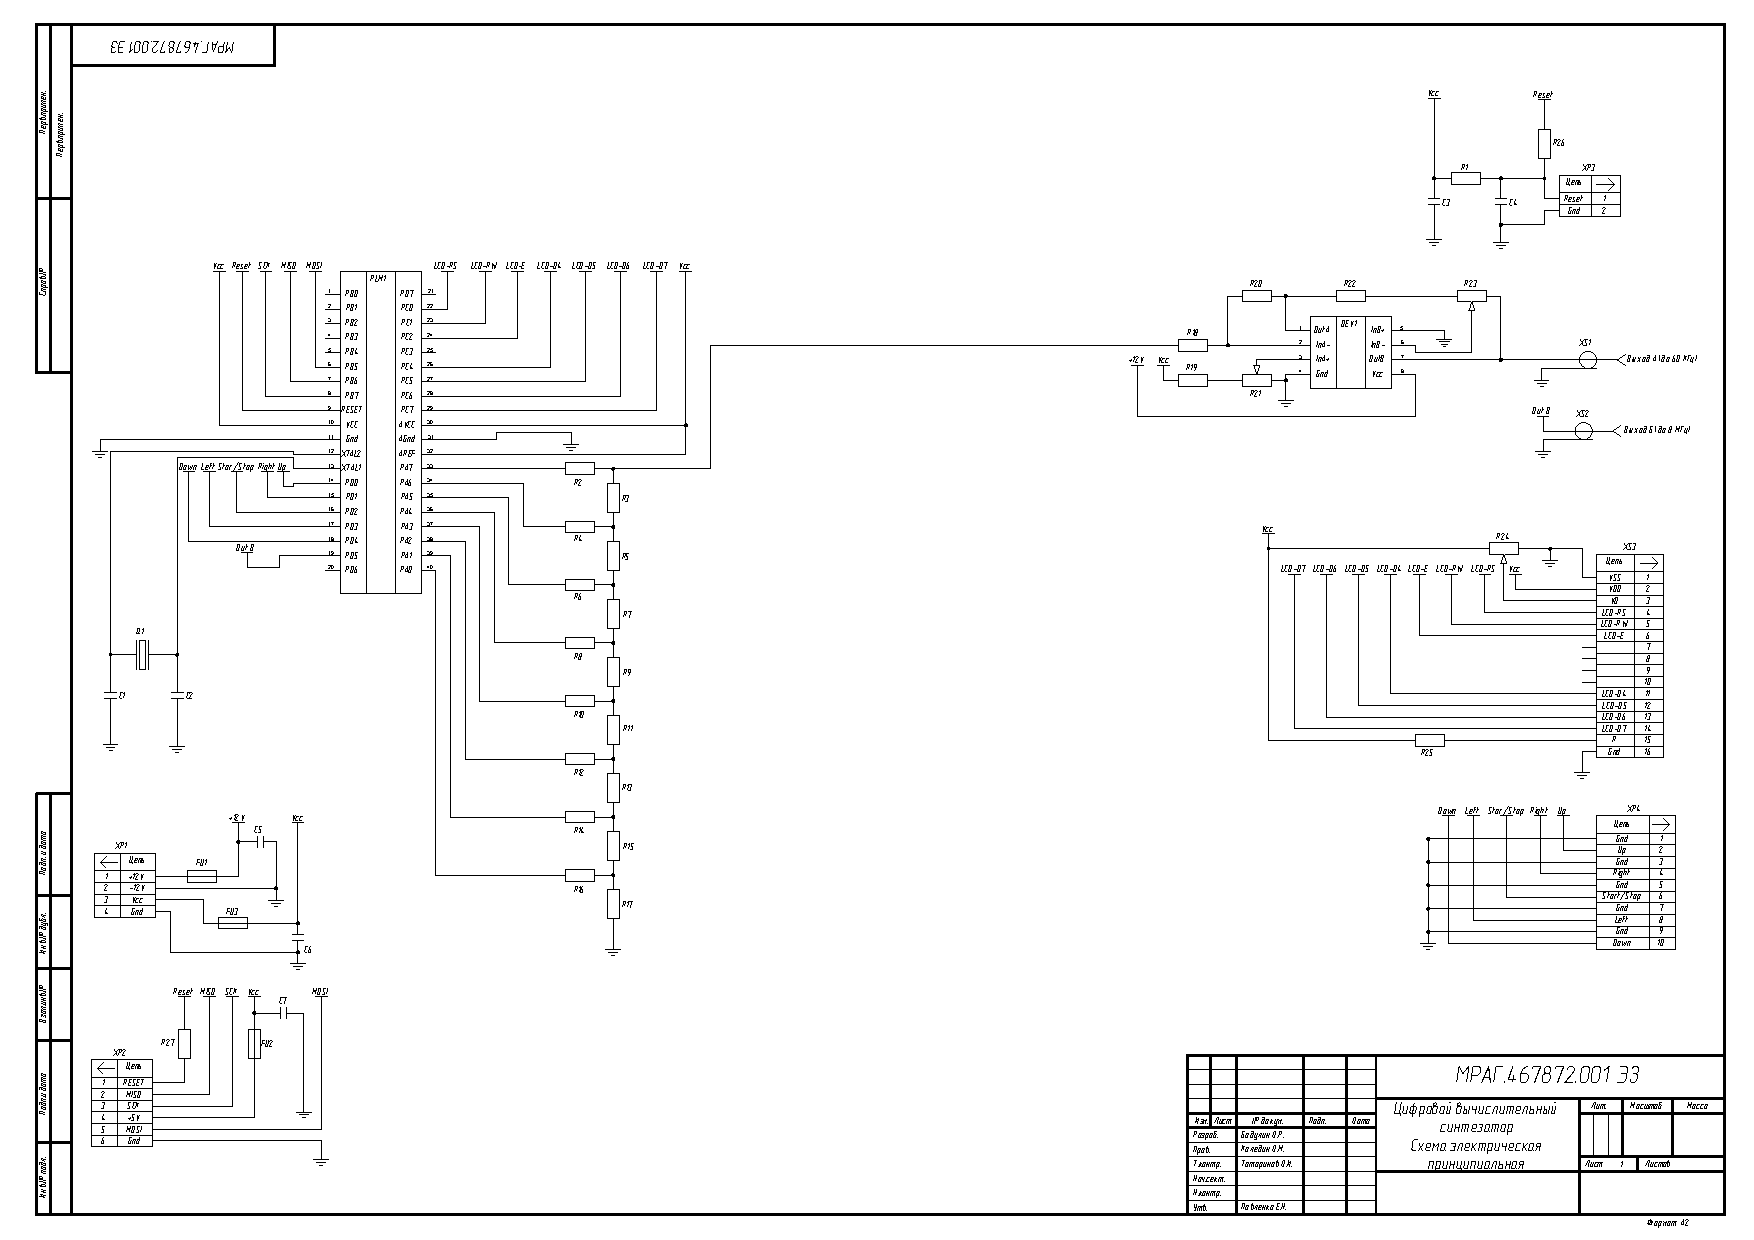
\includepdf[pages = {1}]{app/CD/MRAG.467872.001-EZ.pdf}
%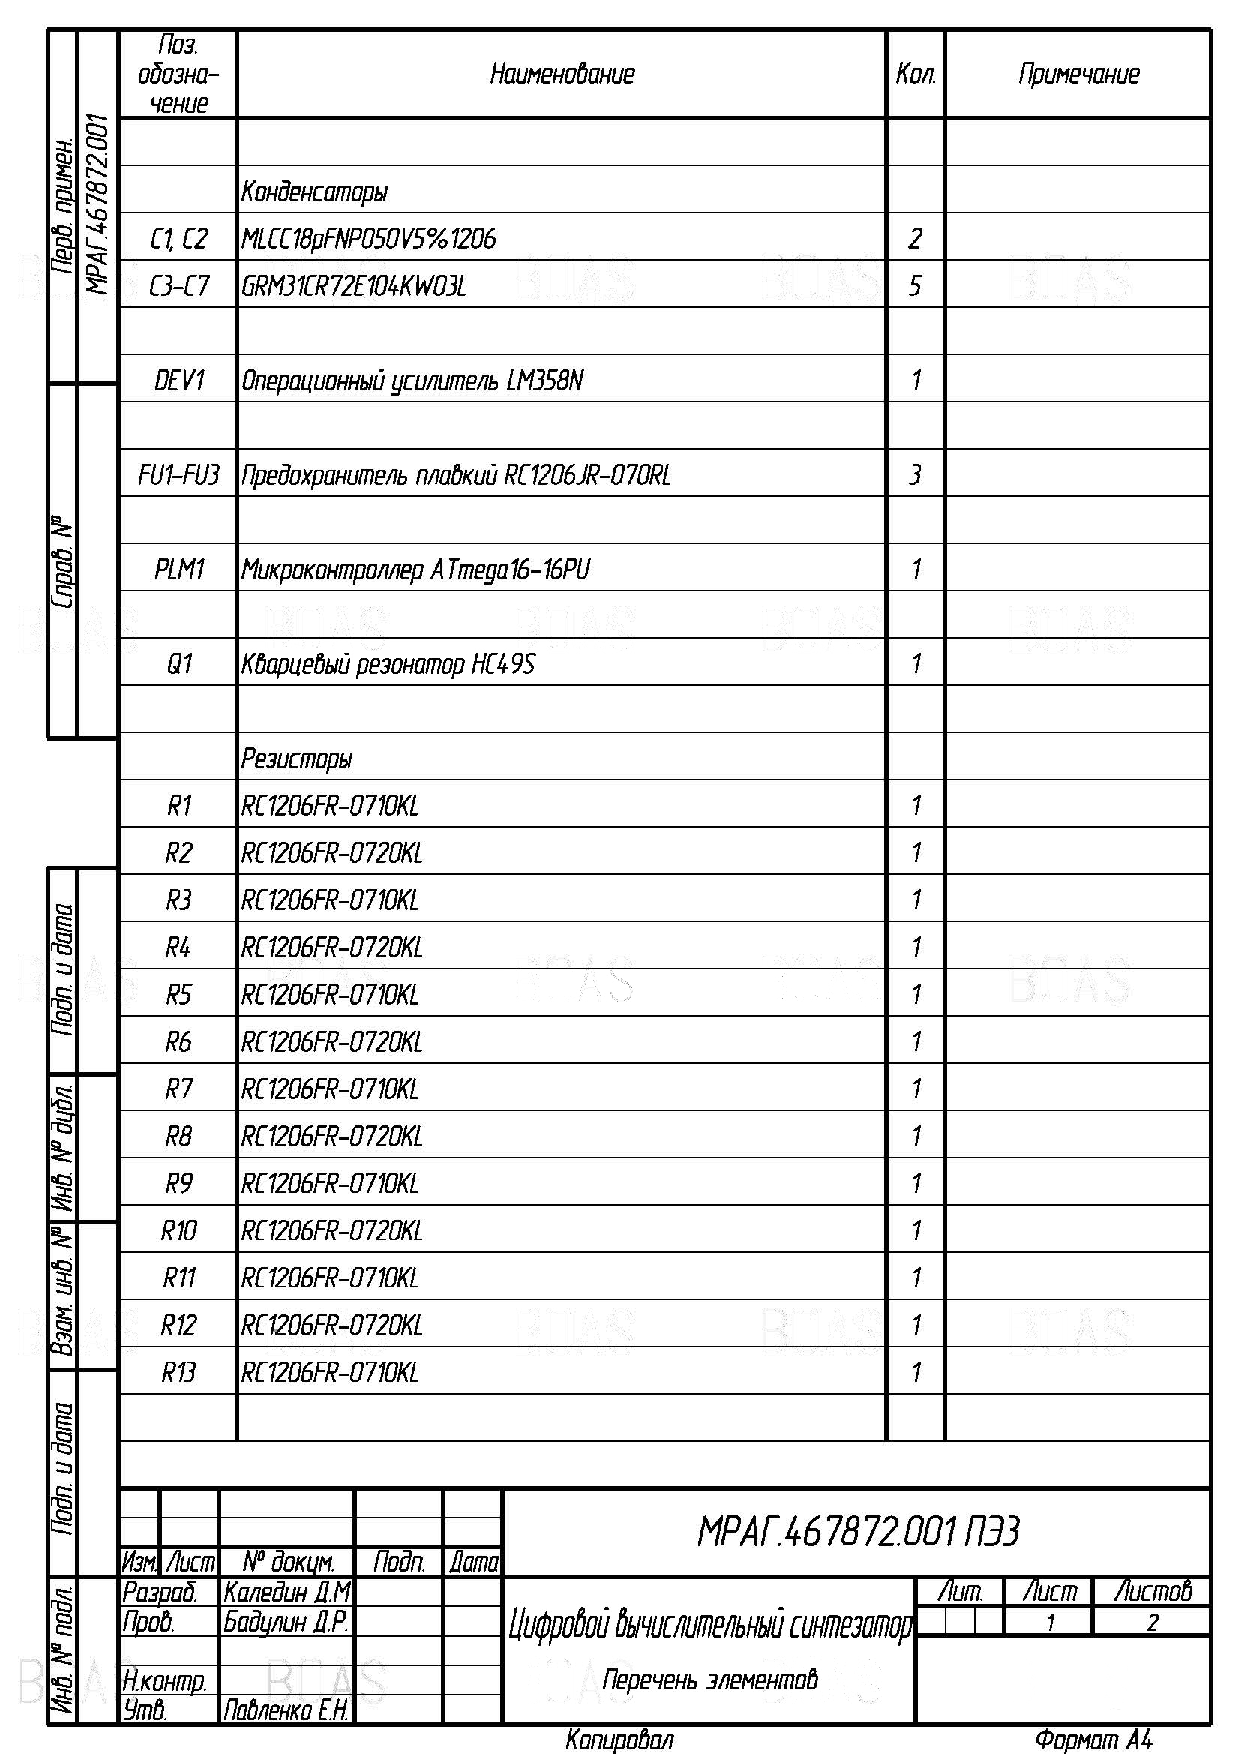
\includepdf[pages = {1,2}]{app/CD/MRAG.467872.001-PE3.pdf}
%\includepdf[pages = {1,2}]{app/CD/MRAG.467872.001-SB.pdf}
%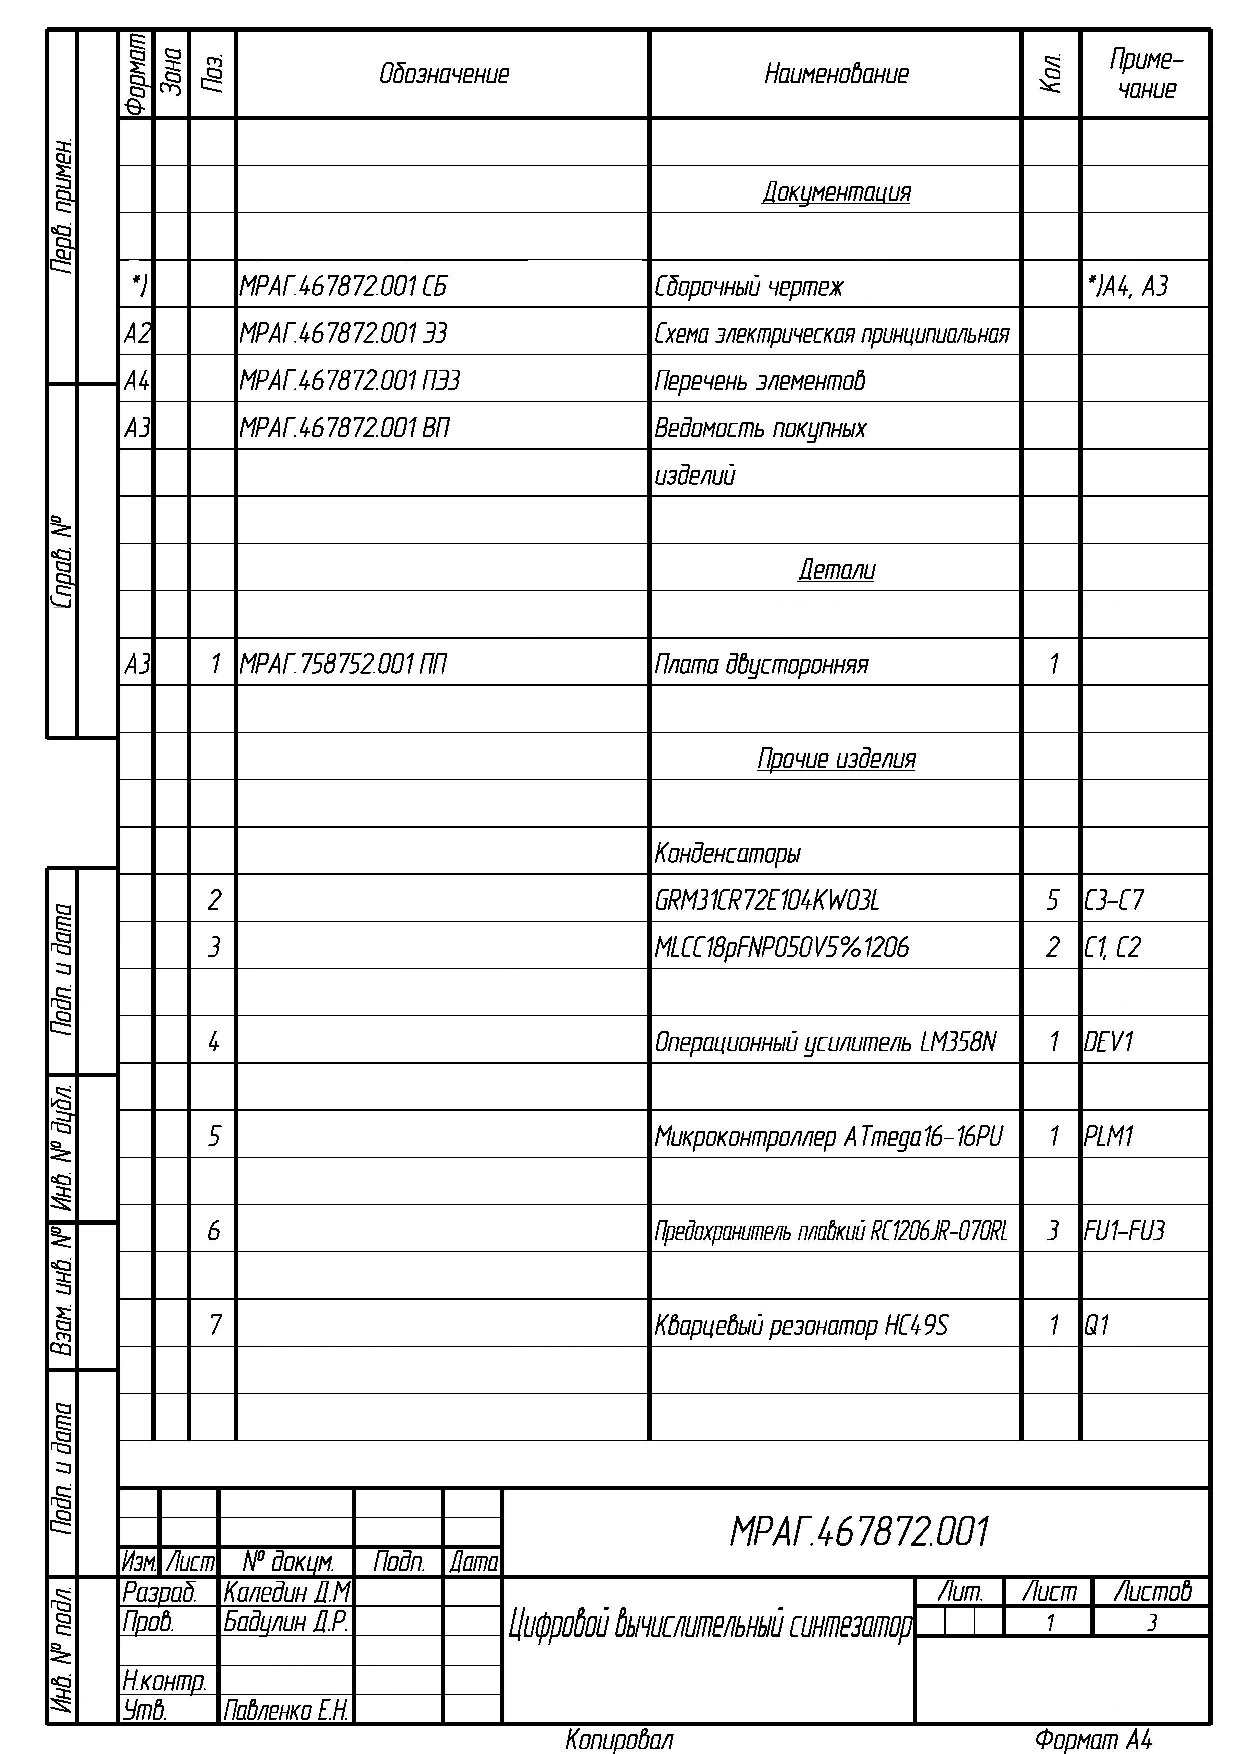
\includepdf[pages = {1,2,3}]{app/CD/MRAG.467872.001.pdf}
%\includepdf[pages = {1,2,3,4,5,6,7,8}]{app/CD/MRAG.758752.001-PP.pdf}
\end{document}
%\newpage
%\appendix{1}
%\section*{Приложение}\label{app:one}
